
Rust is a system programming language which provides memory safety without runtime checking like GC and necessity of explicit memory de/allocation. 
To ensure memory safety, Rust provides restrictive coding patterns and checks lifetime of value and memory safety at compile-time.
The restrictive patterns also enables a developer to write fearless concurrent code that is free of data races.
Main concepts of Memory Management in Rust are ownership, move, and borrowing.

\subsection{Ownership}
In ownership feature or Rust, each value has a variable called owner.
This owner has information about the value, such as location in memory, length and capacity of the value. 
For example, the object representation of Vec$<$i32$>$ is shown in Figure~\ref{fig:rustvec}. The upper boxes represent owner variable in stack frame. 
The lower boxes represent contiguous memory allocated to store i32. Its capacity is specified 10, but 7 values of i32 are stored. 
Therefore, there are still spaces to store 3 values of i32 without reallocation of memory. This owner can live on the scope associated with its lifetime.
When the owner is dropped, the value will be dropped too. This feature is similar to how RAII in C++ works. 
However, acquisition of owner out of the scope where it was constructed is available in Rust with the concept of move. 

\begin{figure}[htb]
    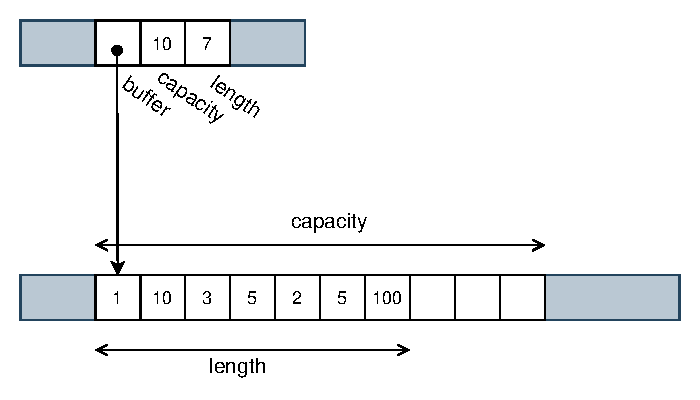
\includegraphics[width=15cm]{rust_vec.eps}
    \caption{Representation of Rust Vec$<$i32$>$}
    \label{fig:rustvec}
\end{figure}


\subsection{Move}
In Rust, for most types of operations like assigning a value to a variable, passing it to a function, or returning it from a function does not copy the value: it moves it. 
With each move, a value can be transferred from one owner to another. The previous variable does not have ownership of the value; it is moved to a newly assigned variable. 
To understand how this assignment implementation is unique from other programing languages, Java, C++, and Rust code example of assigning list or vector of strings are shown.

Below a few lines of code are initialization of list of string and reassigning it to other variables. 
\begin{lstlisting}
    List<String >s = new ArrayList<>(
                     Arrays.asList("lemon", "orange", "apple"))
    List<String> t = s
    List<String> u = s
 \end{lstlisting}
Figure~\ref{fig:javalist} represents the memory allocated after a Java ArrayList of strings is initialized and assigned to variable called s. After assigning s to t and to u, 
the memory representation become Figure~\ref{fig:pythonlistcopied}. The assignments are simply setting pointers to the ArrayList object and increment reference count. 

\begin{figure}[htb]
    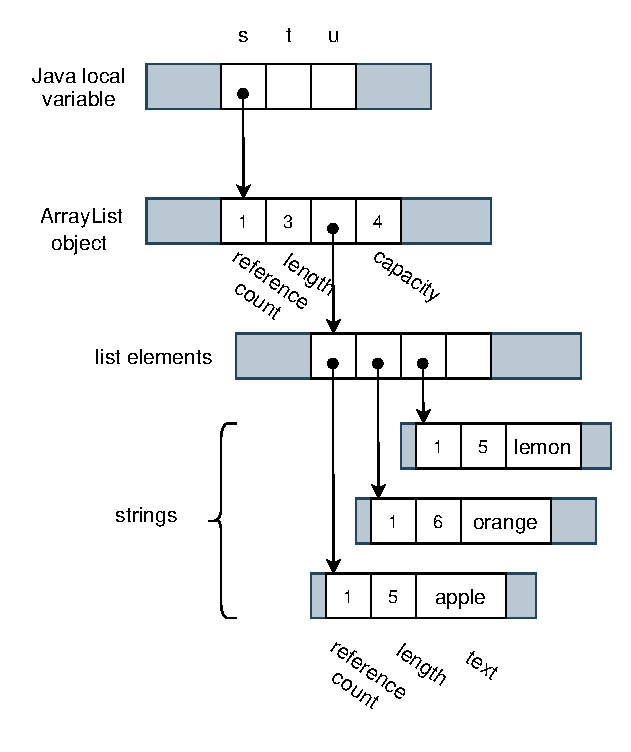
\includegraphics[width=10cm]{java_array.eps}
    \caption{Representation of Java ArrayList of String}
    \label{fig:javalist}
\end{figure}

\begin{figure}[htb]
    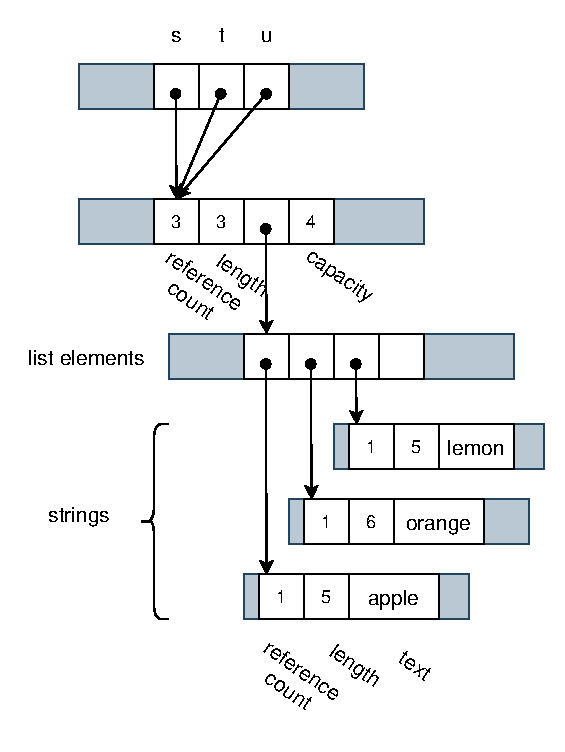
\includegraphics[width=10cm]{python_list.eps}
    \caption{Representation of Java ArrayList of String after assignment to another variable}
    \label{fig:pythonlistcopied}
\end{figure}

Now, the analogous C++ code is shown below. 
\begin{lstlisting}
    vector<string> s = {"lemon", "orange", "apple"};
    vector<string> t = s;
    vector<string> u = s;
 \end{lstlisting}
Figure~\ref{fig:cpluscplusvector} shows the memory allocated when the vector is initialized. Figure~\ref{fig:cpluscplusvectorcopied} is a representation of after the assignments of s to t and to u. 
In C++, assigning value of vector to other variables involves allocating memory for new vector and copying the contents of the original vector to newly allocated one. 

\begin{figure}[htb]
    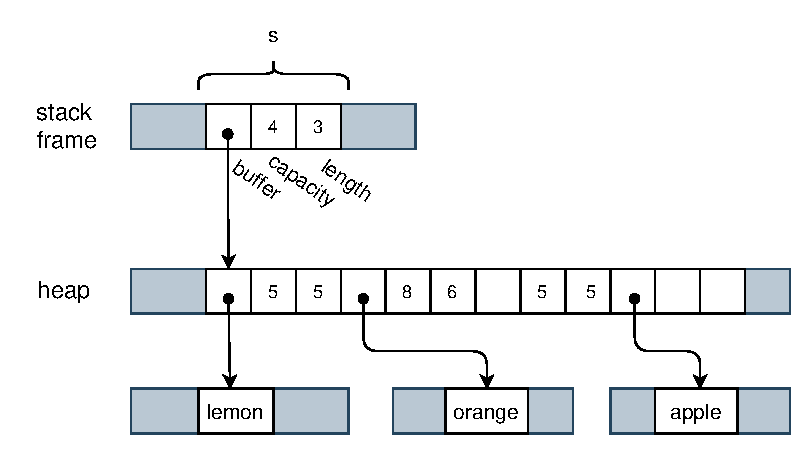
\includegraphics[width=15cm]{cplusplus_vector.eps}
    \caption{Representation of C++ vector of string}
    \label{fig:cpluscplusvector}
\end{figure}


\begin{figure}[htb]
    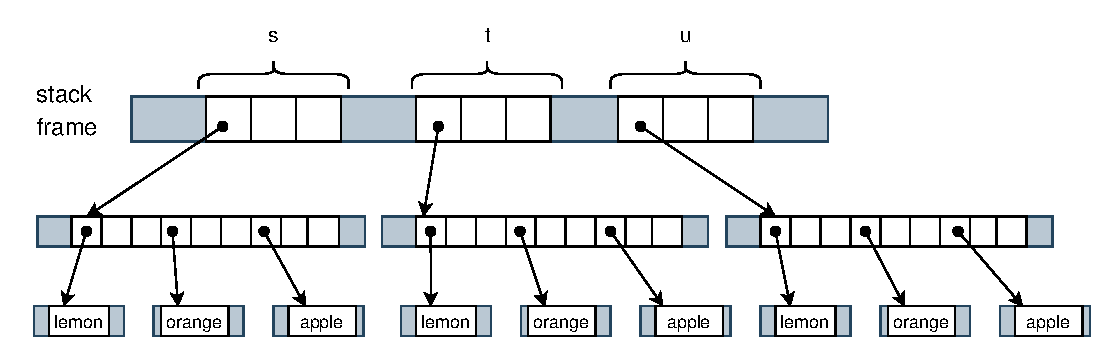
\includegraphics[width=15cm]{cplusplus_vector_copied.eps}
    \caption{Representation of C++ vector of string after assignment to another variable}
    \label{fig:cpluscplusvectorcopied}
\end{figure}


In Rust code, the code is like below, 
\begin{lstlisting}
    let s = vec!["lemon".to_string, "orange".to_string, "apple".to_string];
    let t = s;
    let u = s;
 \end{lstlisting}

The representation of the original Vec of String in Rust is the almost same in C++ vector of string. Figure~\ref{fig:rustvecmoved} however shows different behavior when Rust assigns s to t. 
The value is moved to t from s so that the source variable s is uninitialized. The Rust code actually throws compile error, because we are assigning uninitialized variable at the last line.

\begin{figure}[htb]
    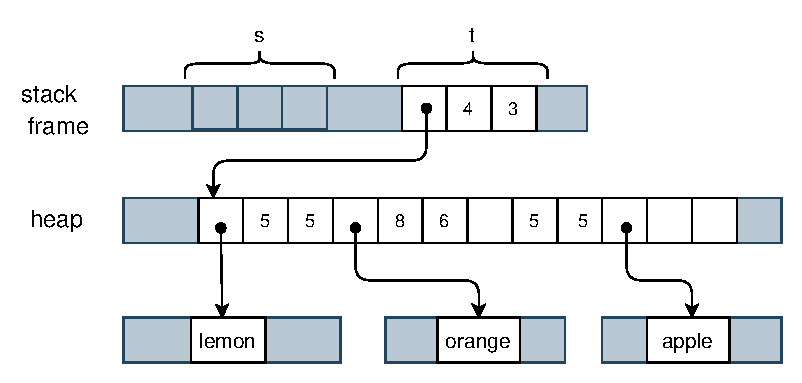
\includegraphics[width=15cm]{rust_vec_moved.eps}
    \caption{Representation of Rust Vec$<$String$>$ after assignment to another variable}
    \label{fig:rustvecmoved}
\end{figure}


\subsection{Borrowing}
Borrowing lets code use a value temporarily without affecting its ownership so that it reduces unnecessary movement of ownership. 
One use case is when value is used in function and needed to be passed to the argument. If the argument takes ownership and the function does not return the value, 
the ownership of value goes out of scope and the memory is deallocated. One can pass reference of the value to the argument instead of owner. 
The reference goes out of scope, but ownership remains the same.
